\documentclass[../main.tex]{subfiles}

\begin{document}

\chapter[Resilient Primal Decomposition-based dMPC for scarce systems]{Resilient \\Primal Decomposition-based \\distributed \\Model Predictive Control\\ for scarce systems}\label{sec:safe_pddmpc_eq}
\epigraph{\centering So you tell me 'trust me' \\I can trust you\\ Just let me show you \\But I gotta work it out in a shadow of doubt \\'Cause I don't know if I know you}
{\textit{Lie}\\\textsc{Kevin Moore}}

In this chapter, we focus on the analysis of the primal decomposition-based \dmpc{} problem for scarce systems when in the presence of the attack chosen in~\S\ref{sec:anomalous}.

With the knowledge acquired after the analysis, we propose a method to detect the attacks and mitigate its effects.

\minitoc


\section{Scarce systems under attack}\label{sec:analys-scarce-syst}

Different from~\cite{VelardeEtAl2018,MaestreEtAl2021} which propose robust solutions, we propose a resilient \dmpc{} based on a hybrid of analytical/learning active detection method.
For this end, we begin with an analysis of the system under attack.

\subsection{Scarce Systems}\label{sec:scarce-systems}
First we recall the monolithic \mpc{} equivalent problem~\eqref{eq:qp_standard_form}, once more reproduced for the reader's convenience,
\begin{equation}
  \label{eq:qp_standard_form_again}
  \tag{\ref*{eq:qp_standard_form}}
  \begin{aligned}
    \begin{matrix}
      \underset{\vec{U}[k]}{\mathrm{minimize}} &
                                                 \frac{1}{2}\norm{\vec{U}[k]}^{2}_{H} + {\vec{f}[k]}^{T}\vec{U}[k] &\\
      \mathrm{subject~ to} &
                             \bar{\Gamma}\vec{U}[k]\preceq {\vec{U}}_{\text{max}}
    \end{matrix}
  \end{aligned},
\end{equation}
and the local problems~\eqref{eq:DOP_local} solved in the primal decomposition, also reproduced,

\begin{equation}
  \label{eq:DOP_local_reprise}
  \tag{\ref*{eq:DOP_local}}
  \bar{J}_{i}^{\star}(\thetaik)=
  \begin{matrix}
    \underset{\vec{U}_{i}[k]}{\mathrm{minimize}}&\obji=\frac{1}{2}\norm{\vec{U}_{i}[k]}^{2}_{H_{i}} + {\vec{f}_{i}[k]}^{T}\vec{U}_{i}[k]\\
    \mathrm{subject~ to} & \bar{\Gamma}_{i}\vec{U}_{i}[k] \preceq \thetaik:\lambdaik
  \end{matrix}.
\end{equation}

The unconstrained version of problems~\eqref{eq:qp_standard_form_again} and~\eqref{eq:DOP_local_reprise} are
\begin{align}
  \label{eq:qp_standard_form_unconstrained}
  \begin{aligned}
    \begin{matrix}
      \underset{\vec{U}[k]}{\mathrm{minimize}} &
                                                 \frac{1}{2}\norm{\vec{U}[k]}^{2}_{H} + {\vec{f}[k]}^{T}\vec{U}[k] &\\
    \end{matrix},
  \end{aligned}\\
  \label{eq:DOP_local_unconstrained}
  \begin{aligned}
    \begin{matrix}
    \underset{\vec{U}_{i}[k]}{\mathrm{minimize}}&\frac{1}{2}\norm{\vec{U}_{i}[k]}^{2}_{H_{i}} + {\vec{f}_{i}[k]}^{T}\vec{U}_{i}[k]\\
    \end{matrix},
  \end{aligned}
\end{align}
and have analytical solutions~\cite{BoydVandenberghe2004}
\begin{align}
  \label{eq:qp_standard_form_unconstrained_solution}
  \vec{U}_{\text{unc}}^{\star}[k]=-H^{-1}\vec{f}[k],\\
  \label{eq:DOP_local_unconstrained_solution}
  \vec{U}_{i_{\text{unc}}}^{\star}[k]=-H_{i}^{-1}\vec{f}_{i}[k].
\end{align}

We call a system scarce when its unconstrained solution $\vec{U}_{\text{unc}}^{\star}[k]$ lies outside the bounds of the polytope formed by the constraints for all $k$, i.e.,
\begin{equation}
\bar{\Gamma}\vec{U}_{\text{unc}}[k]\succ {\vec{U}}_{\text{max}}, \forall k.
\end{equation}

Furthermore, in this chapter, we assume that for all sub-systems, their unconstrained solutions $\vec{U}_{i_{\text{unc}}}^{\star}[k]$ neither respect the local constraints
\begin{equation}
\bar{\Gamma}_{i}\vec{U}_{i_{\text{unc}}}^{\star}[k]\succ \thetaik, \forall i\in\set{M}, \forall k.
\end{equation}

This means that the optimal solution would need more resources (more than $\vec{U}_{\max}$). So the solution of those \qp{} result on the projection of the solutions onto the polytope, which results being projected on the perimter of the polytope.

We assume that given projection solves the inequality constrained problem equivalent to an equality constraint problem
\begin{equation}
  \label{eq:qp_standard_form_equality}
  \begin{aligned}
    \begin{matrix}
      \underset{\vec{U}[k]}{\mathrm{minimize}} &
                                                 \frac{1}{2}\norm{\vec{U}[k]}^{2}_{H} + {\vec{f}[k]}^{T}\vec{U}[k] &\\
      \mathrm{subject~ to} &
                             \bar{\Gamma}\vec{U}[k]= {\vec{U}}_{\text{max}}
    \end{matrix}
  \end{aligned}.
\end{equation}

\begin{remark}
  Observe that this is not always true using the same $\bar{\Gamma}$ (or $\bar{\Gamma}_{i}$).
  The constraints in~\eqref{eq:qp_standard_form_again} and~\eqref{eq:DOP_local_reprise}, can be interpreted as the intersection of the halfspaces described by the rows of $\bar{\Gamma}$ (or $\bar{\Gamma}_{i}$) and $\vec{U}_{\max}$ (or $\thetaik$), i.e., the halfspaces
  ${\set{S}_i=\setbuild{\vec{x}}{\elem[i,\star]{{\bar{\Gamma}}}\vec{x}\leq\elem[i,\star]{\vec{U}_{\max}}}}$, and the intersection ${\set{S}=\setbuild{\vec{x}}{\bar{\Gamma}\vec{x}\preceq\vec{U}_{\max}}=\bigcap\limits_{i=1}^{\card\vec{U}_{\max}}}\set{S}_{i}$ (and conversely for $\bar{\Gamma}_{i}$ and $\thetaik$).

  For this to be true, only the halfspaces closest to the unconstrained solution are kept and transformed into intersection of hyperplanes (equality constraint).
  This computation of active sets and distances may be costly depending on the number of halfspaces used and the dimensions of the variables.

  For our study cases where $\Gamma$ has all its elements positive (such as postive weighted sum of all inputs), and block diagonal structure with repeating pattern (from the \mpc{} definition~\eqref{eq:construction_Gamma}), we assume we can find the corresponding problem and change $\bar{\Gamma}$ (and $\bar{\Gamma}_i$) accordingly, by removing the proper rows.
\end{remark}

As one can perceive, it leads to a decomposition exactly as in \S\ref{sec:example-interpr}
with local problems~\eqref{eq:example_local_problem} and negotiation equation~\eqref{eq:example_projectedSubgradient_lambda}, reproduced here,
\begin{equation}
  \begin{matrix}
  \label{eq:example_local_problem_reprise}
  \tag{\ref*{eq:example_local_problem}}
    \underset{\vec{U}_{i}[k]}{\mathrm{minimize}}&\obji=\frac{1}{2}\norm{\vec{U}_{i}[k]}^{2}_{H_{i}} + {\vec{f}_{i}[k]}^{T}\vec{U}_{i}[k]\\
    \mathrm{subject~ to} & \bar{\Gamma}_{i}\vec{U}_{i}[k] = \thetaik:\lambdaik
  \end{matrix}
\end{equation}
\begin{equation}
  \label{eq:example_projectedSubgradient_lambda_reprise}
  \tag{\ref*{eq:example_projectedSubgradient_lambda}}
 \thetai\pplusone=\thetai\p+\rho\p\left(\lambdai\p-\frac{1}{M}\sum_{j=1}^{M}\vec{\lambda}_j\p\right),\forall i\in\set{M}.
\end{equation}

These are the equations we will use for our analysis.

\subsection{Why scarce systems?}\label{sec:why-scarce-systems}

When a system does not suffer from scarcity, the solution of the unconstrained problem~\eqref{eq:qp_standard_form_unconstrained_solution} respects the inequalities, i.e.,
\begin{equation}
\bar{\Gamma}\vec{U}_{\text{unc}}[k]\preceq {\vec{U}}_{\text{max}},\forall k.
\end{equation}

This way, the elements of $\vec{U}_{\text{unc}}$ lie inside the polytope and none of the constraints is active.
As a consequence, no projection onto the polytope is needed, since it would result on the same point.
That means the solution of the constrained problem is the same as the unconstrained, so the problem is in fact unconstrained.

Instead of needing to solve the local problems~\eqref{eq:DOP_local_reprise} and use a negotiation to decompose the system, the problem doesn't need coordination.
The problem is solved as shown in \S\ref{sec:uncoupled_problems}, i.e., each subsystem solves~\eqref{eq:qp_standard_form_unconstrained_solution} and the solution is already given.

This case is uninteresting because since the agents do not need to compromise to find a consensus, there is no incentive to attack the system to gain more resources since it would not be used and it would not affect the others, who would be nevertheless satisfied.
Furthermore, since no negotiation is needed, there is no communication and the agent would need to find other ways to attack the system.

When the system suffer from scarcity the agents are forced to compete and compromise, what may result in attacks as shown in \S\ref{sec:primal_decomposition} and their dire consequences.

\subsection{Analysis of negotiation}\label{sec:analysis-negotiation}



\begin{enumerate}
  \item Analysis of eigenvalues of negotiation
\end{enumerate}
\begin{equation}
  \begin{matrix}
    \lambdaik=\underset{\lambdaik}{\mathrm{argmax}}\{\underset{\vec{U}_i[k]}{\mathrm{minimize}}\;\frac{1}{2}U_i^TH_iU_i+F_i^TU_i+c_i+\lambda_i^T(U_i-\theta_i^{(p)})\}\\
  \end{matrix}
\end{equation}

\begin{figure}[h]
  \centering
  \begin{subfigure}{.45\textwidth}
    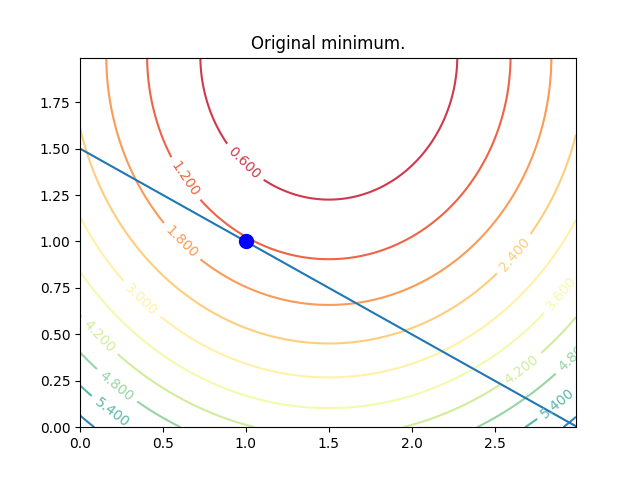
\includegraphics[width=\textwidth]{../img/original-minimum.png}
    \caption{Original minimum.}
    \label{fig:first}
  \end{subfigure}
  \hfill
  \begin{subfigure}{0.45\textwidth}
    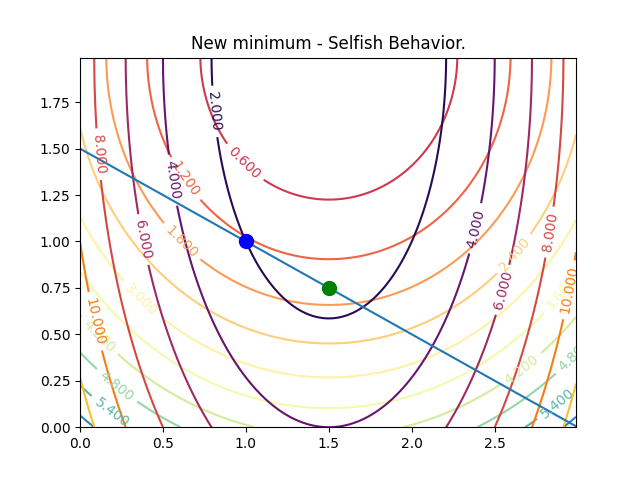
\includegraphics[width=\textwidth]{../img/new-minimum-selfish.png}
    \caption{Minimum after attack.}
    \label{fig:second}
  \end{subfigure}
  \caption{Effects of non-conforming behaviors on optimal value. \todo{Refaire les images}}
  \label{fig:figures}
\end{figure}

\begin{figure}[h]
  \centering
  \begin{subfigure}{0.45\textwidth}
    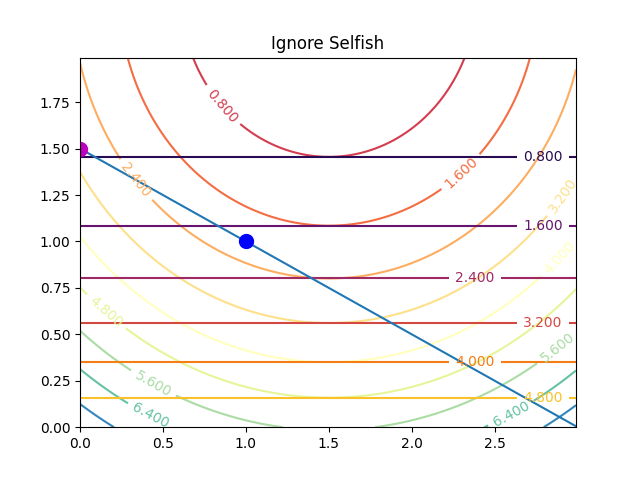
\includegraphics[width=\textwidth]{../img/ignoreX.png}
    \caption{Optimal value after ignoring attacker.}
    \label{fig:third}
  \end{subfigure}
  \hfill
  \begin{subfigure}{0.45\textwidth}
    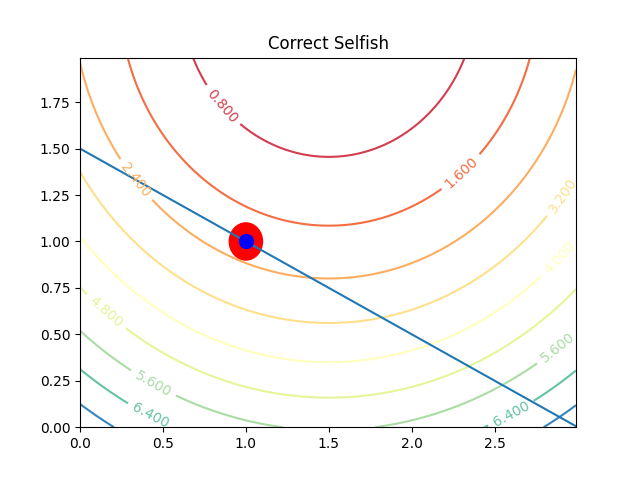
\includegraphics[width=\textwidth]{../img/correctX.png}
    \caption{Optimal value after trying to recover original behavior.}
    \label{fig:third}
  \end{subfigure}

  \caption{Recovery options.}\label{fig:figures}
\end{figure}

\section{Study case}
\label{sec:study-case}

Model 3R-2C \cite{GoudaEtAl2002}
\begin{figure}[h]
  \centering
  \begin{circuitikz}[european]
    \draw (0,0) node[tlground]{} to[isource, l=$P^{\text{heat}}$] ++(0,2) to[short, -*] ++(1.5,0) coordinate (a);

    \draw (a) node[above]{$T^{\text{in}}$}  to[C=$C^{\text{air}}$] ++(0,-2) node[tlground]{};
    \draw (0,-3) node[tlground]{} to[isource, l=$I^{\text{sol}}$] ++(0,2)
    to[short, -*] ++(1.5,0) coordinate (b);
    \draw (b) to[C=$C^{\text{walls}}$] ++(0,-2) node[tlground]{};

    \draw (a) -- ++(2,0) coordinate (c) -- ++(0,-.5) to[R=$R^{\text{iw/ia}}$] ++(0,-2) -- ++(0,-.5) coordinate (d);

    \draw (b) node[above]{$T^{\text{walls}}$} to[short,-*] (d);

    \draw (c) --  ++(2.5,0) -- ++(0,-.5) to[R=$R^{\text{oa/ia}}$] ++(0,-2) -- ++(0,-.5) coordinate (e);

    \draw (d) to[R=$R^{\text{ow/oa}}$] (e) to[battery,l=$T^{\text{out}}$] ++(0,-2) node[tlground]{};
  \end{circuitikz}
  \caption{Thermic Model 3R-2C of a room.}
  \label{fig:3R2C_model}
\end{figure}

The state-space model of each subsystem is given by:
\begin{equation}
  \begin{matrix}
    \label{eq:systems_cont}
    \dot{\vec{x}}_{i}(t)  &=&{A_{c}}_{i}\vec{x}_{i}(t) &+& {B_{c}}_{i}\vec{u}_{i}(t)\\
    \vec{y}_{i}(t)        &=&{C_{c}}_{i}\vec{x}_{i}(t) &&
  \end{matrix},
\end{equation}
where
\begin{equation}
  \label{eq:4}
  \begin{matrix}
    A_{\mathrm{c}_{i}}=\left[
    \begin{matrix}
      -\frac{1}{C^{\text{walls}}_{i}R^{\text{oa/ia}}_{i}}-\frac{1}{C^{\text{walls}}_{i}R^{\text{iw/ia}}_{i}}& \frac{1}{C^{\text{walls}}_{i}R^{\text{iw/ia}}_{i}}\\
      \frac{1}{C^{\text{air}}_{i}R^{\text{iw/ia}}_{i}} &-\frac{1}{C^{\text{air}}_{i}R^{\text{ow/oa}}o_{i}}-\frac{1}{C^{\text{air}}_{i}R^{\text{iw/ia}}_{i}}
    \end{matrix}\right]\\
    \begin{matrix}
      B_{\mathrm{c}_{i}}=\left[
      \begin{matrix}  \frac{10}{C^{\text{walls}}_{i}}& 0\end{matrix}
                                                       \right]\T&C_{\mathrm{c}_{i}}=\left[\begin{matrix}1 & 0\end{matrix}\right]
    \end{matrix}
  \end{matrix}
\end{equation}
where ${\vec{x}_{i}=[{{x}_{A}}_{i}\T\ {{x}_{W}}_{i}\T]\T}$. ${x_A}_i$ and ${x_W}_i$ are the mean temperatures of the air and walls inside room~$i$. $\vec{u}_{i}$ is the input (the heating power)
for the corresponding room. The inputs are constraint by ${\sum_{i=1}^{4}\vec{u}_{i}(t)\preceq 4\mathrm{kW}}$.

\begin{table}[b]
  \centering
  \caption{Model Parameters}\label{tab:modelParamMeaning}
  \begin{tabular}[b]{cl}
    \toprule
    Symbol&Meaning\\
    \midrule
    $C^{\text{air}}_{i}$  &Heat Capacity of Inside Air\\
    $C^{\text{walls}}_{i}$ &Heat Capacity of External Walls\\
    $R^{\text{iw/ia}}_{i}$ &Resist. Between Inside Air and Inside Walls\\
    $R^{\text{ow/oa}}_{i}$ &Resist. Between Outside Air and Outside Walls\\
    $R^{\text{oa/ia}}_{i}$ &Resist. Between Inside and Out.\ Air (from windows)\\
    \bottomrule
  \end{tabular}
\end{table}

\begin{table}[b]
  \centering
  \caption{
    Parameters for each agent}\label{tab:modelParam}
  \begin{tabular}[t]{cccccc} \toprule
    Symbol& I & II & III & IV &Unit\\
    \midrule
    $C^{\text{walls}}$   &$5.4$&$4.9$&$4.7$&$4.7$ &$10^{4}\mathrm{J/K}$ \\
    $C^{\text{air}}$     &$7.5$ &$8.4 $&$8.2$ &$7.7$&$10^{4}\mathrm{J/K}$  \\
    $R^{\text{oa/ia}}$   &$5.2$&$4.6$&$4.9$&$5.4$&$10^{-3}\mathrm{K/W}$ \\
    $R^{\text{iw/ia}}$   &$2.3$&$2.4$&$2.3$&$2.9$&$10^{-4}\mathrm{K/W}$\\
    $R^{\text{ow/oa}}$   &$1.5$&$0.6$&$0.7$&$0.7$& $10^{-4}\mathrm{K/W}$ \\
    \bottomrule
  \end{tabular}
\end{table}

the attacker has no motivation to get more

\end{document}
